\documentclass{article}
\usepackage[utf8]{inputenc}
\usepackage[T1]{fontenc}
\usepackage{booktabs}
\usepackage{graphicx}
\usepackage[margin=1in]{geometry}

\title{RGAT com mais épocas de treino: revisão da hipótese de sub-treino}
\author{}
\date{}

\begin{document}
\maketitle

\section{Motivação}

\texttt{estudo/scibench\_ablation.tex} concluiu, a partir de quatro
comparações controladas (2 tamanhos de modelo $\times$ 2 benchmarks,
todas com 3 épocas de treino), que o RGAT nunca supera sua contraparte
T5 pura do mesmo tamanho. Antes de aceitar essa conclusão como
definitiva, testamos a hipótese mais óbvia de confusão: será que 3
épocas simplesmente não são treino suficiente para uma arquitetura que
adiciona camadas de atenção sobre grafo inicializadas do zero (o RGAT
não tem pré-treino próprio, ao contrário do backbone T5)? Se o RGAT
precisa de mais gradiente para as camadas novas convergirem, o
resultado anterior mediria sub-treino, não uma limitação real da
arquitetura.

Para testar isso, re-treinamos as duas configurações com RGAT no
ScienceBenchmark por \textbf{10 épocas} (mesmos dados, mesmos
hiperparâmetros de \emph{learning rate}/otimizador/\emph{batch}
efetivo das rodadas de 3 épocas -- único fator alterado é
\texttt{num\_train\_epochs}):

\begin{itemize}
\item \textbf{t5-small + RGAT}: \texttt{graphix-scibench-t5small-rgat-10ep}
\item \textbf{t5-base + RGAT completo} (+oncomx, \emph{gradient checkpointing}):
      \texttt{graphix-scibench-finetune-gc-10ep}
\end{itemize}

\section{Resultado principal}

\begin{table}[h]
\centering
\caption{Comparação 3 épocas vs.\ 10 épocas (melhor checkpoint por eval\_loss), dev set do ScienceBenchmark.}
\label{tab:more-epochs}
\begin{tabular}{lrrrr}
\toprule
\textbf{Configuração} & \textbf{eval\_loss} & \textbf{exact match} & \textbf{exec} & \textbf{tempo de treino} \\
\midrule
t5-small + RGAT, 3 épocas   & 1,1517 & 1,04\% & 0,68\% & 3h46min \\
t5-small + RGAT, 10 épocas  & \textbf{0,9243} & \textbf{5,19\%} & \textbf{4,10\%} & 6h59min \\
\midrule
t5-base + RGAT completo, 3 épocas  & 1,6765 & 0,0\% & 0,34\% & 9h42min \\
t5-base + RGAT completo, 10 épocas & \textbf{1,4567} & 0,0\% & \textbf{2,73\%} & 16h13min \\
\bottomrule
\end{tabular}
\end{table}

\textbf{O achado é inequívoco: mais épocas melhoram substancialmente o
RGAT em ambos os tamanhos de modelo.} A Figura~\ref{fig:curves} mostra
que a melhora não satura nas 3 épocas originais -- pelo contrário, o
\emph{eval\_loss} de ambos os modelos continua caindo de forma quase
monotônica até a época 9--10, e a \emph{execution accuracy} sobe junto
(com ruído normal de treino, mas sem sinal de platô).

\begin{itemize}
\item \textbf{t5-small + RGAT}: eval\_loss caiu 20\% (1,15 $\to$ 0,92),
      exec subiu $\mathbf{6\times}$ (0,68\% $\to$ 4,10\%) e exact match
      subiu $5\times$ (1,04\% $\to$ 5,19\%).
\item \textbf{t5-base + RGAT completo}: eval\_loss caiu 13\%
      (1,68 $\to$ 1,46), exec subiu $\mathbf{8\times}$
      (0,34\% $\to$ 2,73\%). Exact match permanece em 0\% nas duas
      durações de treino.
\end{itemize}

\begin{figure}[h]
\centering
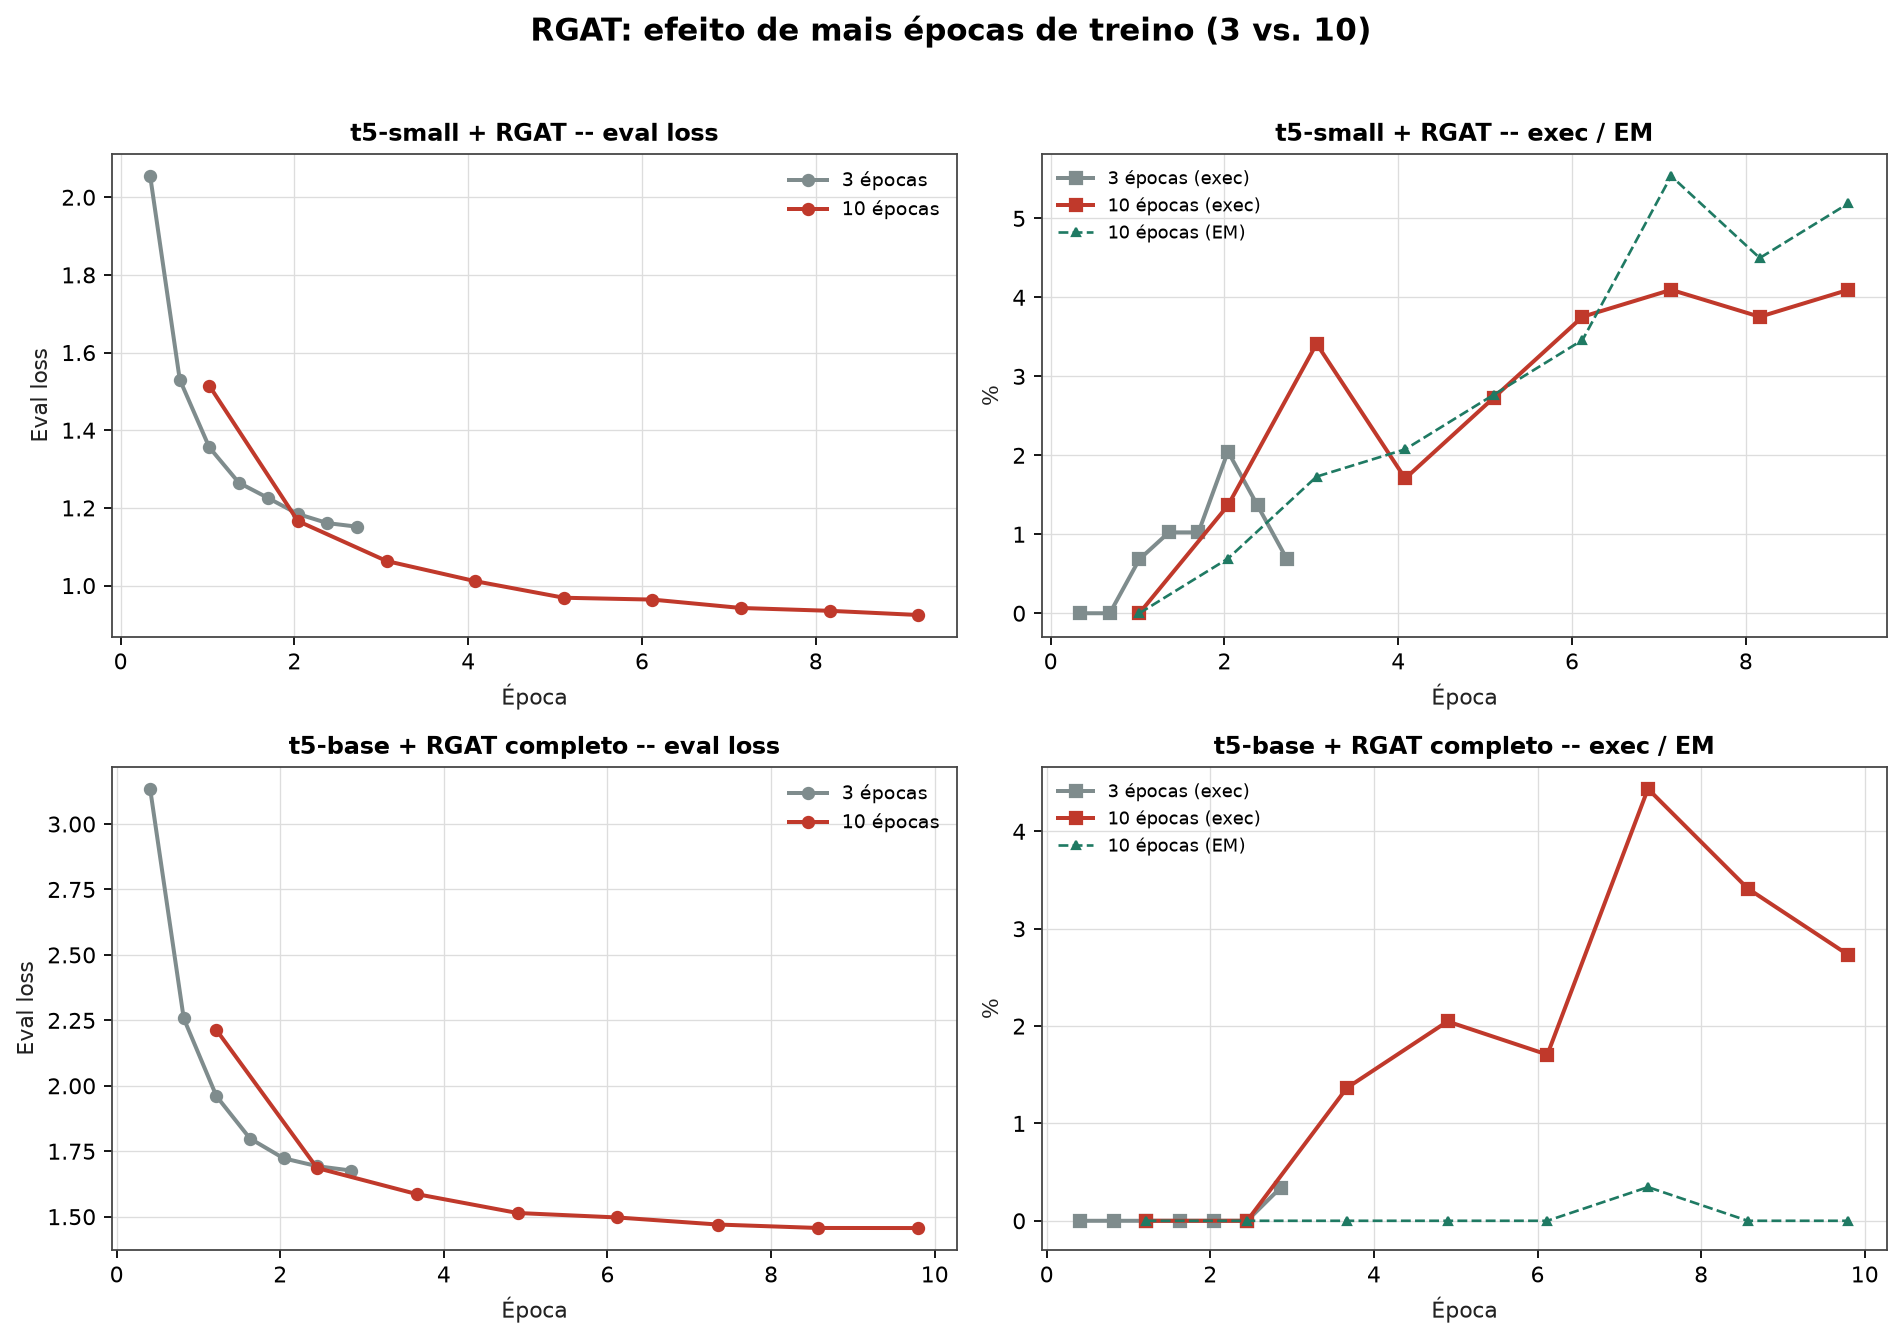
\includegraphics[width=0.95\textwidth]{more_epochs_ablation_curves.png}
\caption{Eval loss e métricas discretas por época, 3 vs.\ 10 épocas, para os dois modelos com RGAT.}
\label{fig:curves}
\end{figure}

\begin{figure}[h]
\centering
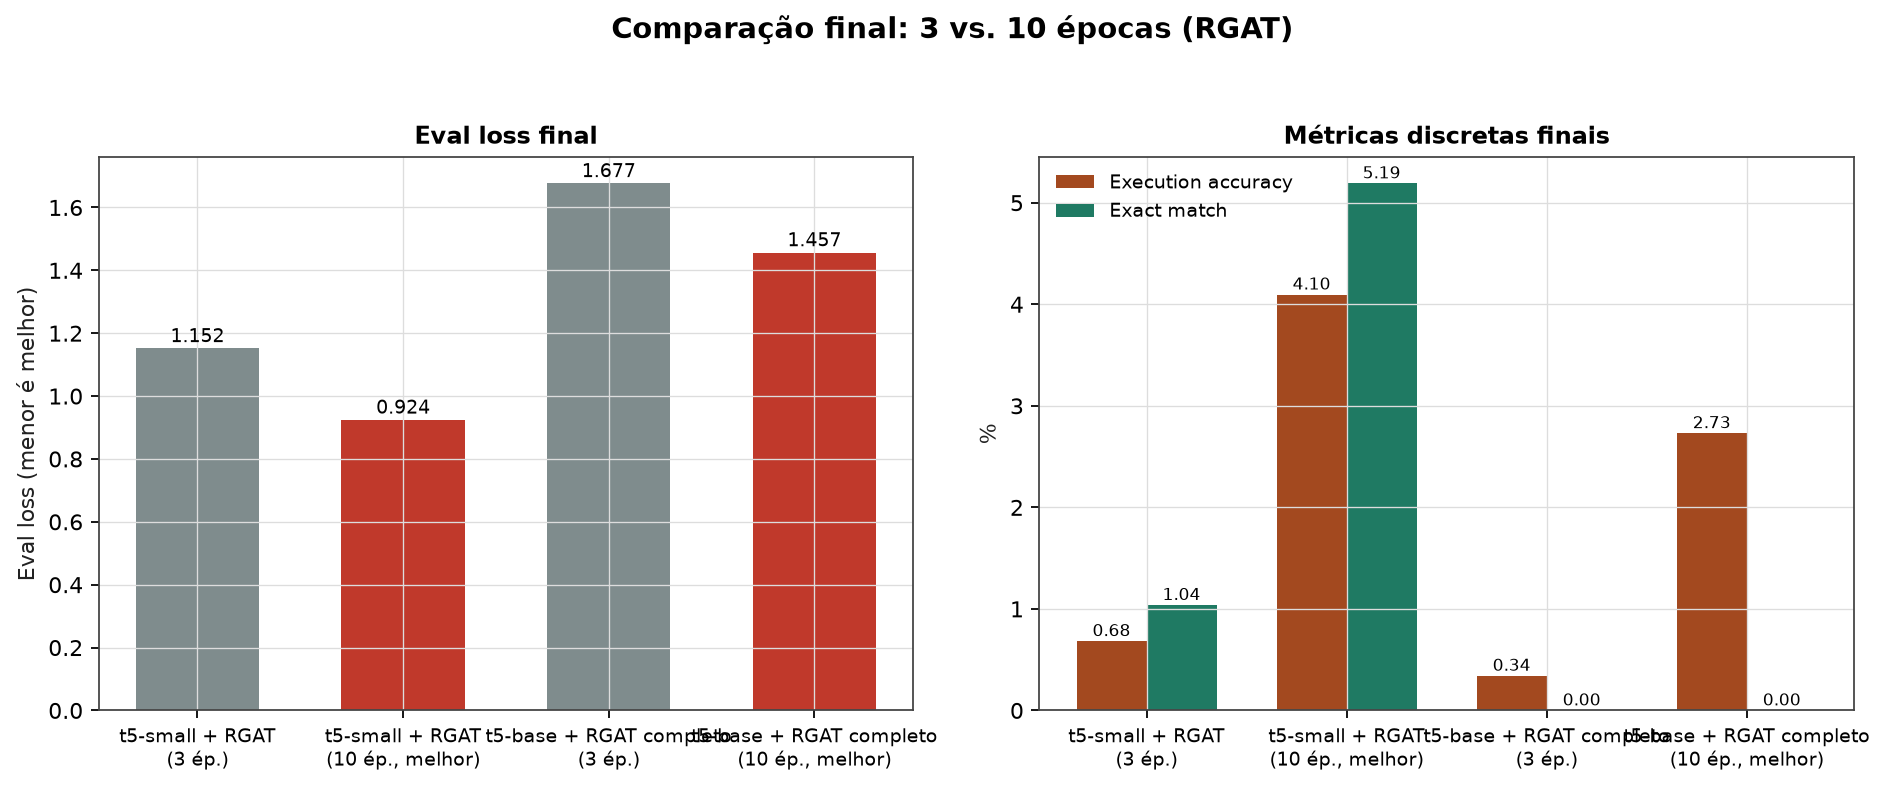
\includegraphics[width=0.95\textwidth]{more_epochs_ablation_summary.png}
\caption{Comparação final (melhor checkpoint) entre as quatro rodadas.}
\label{fig:summary}
\end{figure}

\section{O que isso muda na conclusão anterior}

A conclusão de \texttt{estudo/scibench\_ablation.tex} -- ``o RGAT nunca
vence sua contraparte do mesmo tamanho'' -- \textbf{precisa ser
matizada, não descartada}. Dois pontos ficam mais claros agora:

\textbf{1. Sub-treino era parte real da explicação.} Com apenas 3
épocas, o RGAT estava genuinamente longe de convergir: suas camadas de
atenção sobre grafo, inicializadas do zero, exigem mais passos de
gradiente que o backbone T5 pré-treinado para chegar perto de um bom
ponto de operação. Isso não era visível na comparação de 3 épocas
porque não havia uma segunda duração de treino para contrastar --
descartar essa hipótese sem testá-la teria sido prematuro.

\textbf{2. Mesmo com 10 épocas, o RGAT continua atrás do T5 puro.}
Comparando com o t5-base sem RGAT (Tabela~1 de
\texttt{estudo/scibench\_ablation.tex}: exec 8,19\%, treinado em
apenas 3 épocas), o t5-base + RGAT completo com 10 épocas
(exec 2,73\%) ainda fica bem atrás -- e treinou mais que o
\emph{dobro} do tempo (16h13 vs.\ 4h13) para chegar lá. Ou seja: mais
treino claramente ajuda o RGAT, mas não fecha a lacuna para o T5 puro
dentro do orçamento testado. Não podemos afirmar que o RGAT alcançaria
ou superaria o T5 puro com treino ainda mais longo -- apenas que a
comparação de 3 épocas subestimava o potencial do RGAT, e que a
arquitetura continua exigindo mais recursos computacionais por unidade
de ganho do que o T5 puro nesta tarefa e neste regime de dados.

\textbf{Conclusão revisada:} ``RGAT precisa de mais treino'' é
\textbf{confirmado} como fator real -- não é apenas uma hipótese
descartável. Mas ``RGAT supera T5 puro'' continua \textbf{não
confirmado} mesmo com o triplo de épocas; o gargalo observado
originalmente é uma combinação de sub-treino (agora corrigido em
parte) e um custo-benefício computacional que ainda favorece o T5 puro
neste conjunto de experimentos.

\end{document}
